%%%%%%%%%%%%%%%%%%%%%%%%%%%%%%%%%%%%%%%%%%%%%%%%%%%%%%%%%%%%%%%%%%%%
%% I, the copyright holder of this work, release this work into the
%% public domain. This applies worldwide. In some countries this may
%% not be legally possible; if so: I grant anyone the right to use
%% this work for any purpose, without any conditions, unless such
%% conditions are required by law.
%%%%%%%%%%%%%%%%%%%%%%%%%%%%%%%%%%%%%%%%%%%%%%%%%%%%%%%%%%%%%%%%%%%%

\documentclass[
  digital,     %% The `digital` option enables the default options for the
               %% digital version of a document. Replace with `printed`
               %% to enable the default options for the printed version
               %% of a document.
%%  color,       %% Uncomment these lines (by removing the %% at the
%%               %% beginning) to use color in the printed version of your
%%               %% document
  oneside,     %% The `oneside` option enables one-sided typesetting,
               %% which is preferred if you are only going to submit a
               %% digital version of your thesis. Replace with `twoside`
               %% for double-sided typesetting if you are planning to
               %% also print your thesis. For double-sided typesetting,
               %% use at least 120 g/m² paper to prevent show-through.
  nosansbold,  %% The `nosansbold` option prevents the use of the
               %% sans-serif type face for bold text. Replace with
               %% `sansbold` to use sans-serif type face for bold text.
  nocolorbold, %% The `nocolorbold` option disables the usage of the
               %% blue color for bold text, instead using black. Replace
               %% with `colorbold` to use blue for bold text.
  lof,         %% The `lof` option prints the List of Figures. Replace
               %% with `nolof` to hide the List of Figures.
  lot,         %% The `lot` option prints the List of Tables. Replace
               %% with `nolot` to hide the List of Tables.
]{fithesis4}
%% The following section sets up the locales used in the thesis.
\usepackage[resetfonts]{cmap} %% We need to load the T2A font encoding
\usepackage[T1,T2A]{fontenc}  %% to use the Cyrillic fonts with Russian texts.
\usepackage[
  main=english, %% By using `czech` or `slovak` as the main locale
                %% instead of `english`, you can typeset the thesis
                %% in either Czech or Slovak, respectively.
  english, german, czech, slovak %% The additional keys allow
]{babel}        %% foreign texts to be typeset as follows:
%%
%%   \begin{otherlanguage}{german}  ... \end{otherlanguage}
%%   \begin{otherlanguage}{czech}   ... \end{otherlanguage}
%%   \begin{otherlanguage}{slovak}  ... \end{otherlanguage}
%%
%%
%% The following section sets up the metadata of the thesis.
\thesissetup{
    date        = \the\year/\the\month/\the\day,
    university  = mu,
    faculty     = fi,
    type        = mgr,
    department  = Department of Machine Learning and Data Processing,
    author      = Bruno Petrus,
    gender      = m,
    advisor     = {Prof. RNDr. John Smith, CSc.},
    title       = {Segmentation of tunneling nanotubes},
    TeXtitle    = {The Proof of $\mathsf{P}=\mathsf{NP}$},
    keywords    = {keyword1, keyword2, ...},
    TeXkeywords = {keyword1, keyword2, \ldots},
    abstract    = {%
      This is the abstract of my thesis, which can

      span multiple paragraphs.
    },
    thanks      = {%
      These are the acknowledgements for my thesis, which can

      span multiple paragraphs.
    },
    bib         = biblio.bib,
    %% Remove the following line to use the JVS 2018 faculty logo.
    facultyLogo = fithesis-fi,
}
\usepackage{makeidx}      %% The `makeidx` package contains
\makeindex                %% helper commands for index typesetting.
%% These additional packages are used within the document:
\usepackage{paralist} %% Compact list environments
\usepackage{amsmath}  %% Mathematics
\usepackage{amsthm}
\usepackage{amsfonts}
\usepackage{url}      %% Hyperlinks
\usepackage{markdown} %% Lightweight markup
\usepackage{listings} %% Source code highlighting
\lstset{
  basicstyle      = \ttfamily,
  identifierstyle = \color{black},
  keywordstyle    = \color{blue},
  keywordstyle    = {[2]\color{cyan}},
  keywordstyle    = {[3]\color{olive}},
  stringstyle     = \color{teal},
  commentstyle    = \itshape\color{magenta},
  breaklines      = true,
}
\usepackage{floatrow} %% Putting captions above tables
\floatsetup[table]{capposition=top}
\usepackage[babel]{csquotes} %% Context-sensitive quotation marks
\begin{document}
%% The \chapter* command can be used to produce unnumbered chapters:
\chapter*{Introduction}
%% Unlike \chapter, \chapter* does not update the headings and does not
%% enter the chapter to the table of contents. I we want correct
%% headings and a table of contents entry, we must add them manually:
\markright{\textsc{Introduction}}
\addcontentsline{toc}{chapter}{Introduction}

Theses are rumoured to be \enquote{the capstones of education}, so
I decided to write one of my own. If all goes well, I will soon
have a diploma under my belt. Wish me luck!

\chapter{Data}

Our work begun when the Estonian partners send us the four different datasets of
the wanted to study phenomena. To study the effects of tunneling nanotubes which
are these thin, long and often time curved structures, they deciced to use wings
of fly larvae. A schematic can be viewed in Figure [TODO]. This is quite
interesting sample as it generaly has, as can be seen in Figure [TODO] and
[TODO] two distinct layers of cells, between which a vertical pillar like
structures are visible. These structures are what we will refer to in this work
as pillars for simplicity. These belong to the [FINISH] part of the wings. How
such data can be acquired and for more information of the process I recommend
looking into the \parencite{Tran2024Programmed} paper.

The data was captured using fluorescence microscopy. [TODO simple explanation]
and four distinct datasets were acquired. Three of these datasets were captured
with two different channels, larger volume and smaller spatial resolution. All
the datasets are actually part of a time series. The 

The last dataset contains just one channel. The fluorescent dye was selected to
highligh both the pillars and the tunnels as can be seen in Figure [TODO]. As we
can see unlike the previous datasets this was capture at much higher spatial
resolution; therefore, we can see that the dye react mostly in the cell membrane
and they appear hollow. Moreover, the tunnels are much more visible compared to
the previous three datasets, but it only contains a single channel now.

As said before the data was captured by our Estonian partners at [TODO], to
further propel the research they promised us to annotate the three large
datasets, but after several months no labels were given which complicated the
research and work. Hence, we approached our collegues at [TODO what fac.] and
they were kind enough to help us.

\begin{figure}
    \begin{center}
        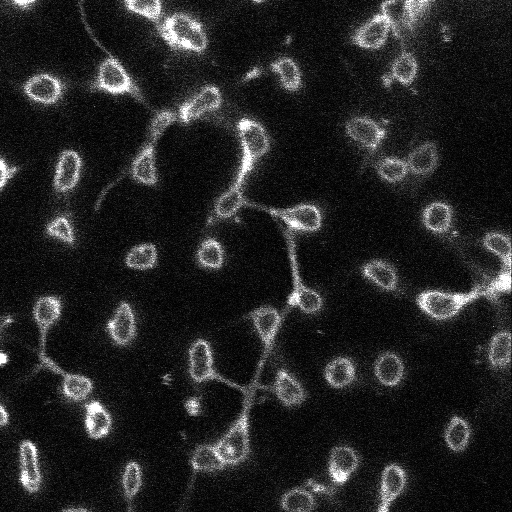
\includegraphics[width=0.6\linewidth]{resources/t017z0_saturated1percent.png}
    \end{center}
    \caption{First slice of the data at time step 17, after the biologist
    preprocessing pipeline}.
    \label{fig:biologistpreprocessing}
\end{figure}

The biologist created a protocol which they followed by annotating the samples.
They decided to preprocess the data by converting the images from 16bit
grayscale image into 8bit grayscale images, then a 1\%-percentile stretch was
applied to further enhance the images. The result of the preprocessing is
visible in Figure \ref{fig:biologistpreprocessing}. As can be seen on the figure,
this makes the tunnels easier to see at the cost making noise more visible.

After the preprocessing is done, the protocol states that picking random time
slots at least 100 instances of tunnels must be fully annotated and 

\chapter{Processing data}
splitting and stuff

\chapter{Architectures}
introduce the various arch

\chapter{Training}
how the neural networks were trained.

\chapter{Evaluation}
how we evaluate the networks

\chapter{Ablation studies}

\chapter{Implementation}

\chapter{Discussion}
what to do next

\end{document}
